% Define block styles
\tikzstyle{block} = [draw, rectangle, text centered, text width=10em, minimum height=0.5em, rounded corners=true]
\tikzstyle{arrowtext} = [text width=4em, text centered]
\tikzstyle{background} = [draw, rectangle, text centered, text width=3.5cm, minimum height=3.5cm, color=white]
\tikzstyle{arrow} = [draw, -latex]

\definecolor{red1}{RGB}{160,0,0}
\definecolor{green1}{RGB}{0,160,0}
\definecolor{blue1}{RGB}{0,0,160}
\definecolor{black}{RGB}{0,0,0}
\definecolor{white}{RGB}{255,255,255}

\usetikzlibrary{shapes.geometric,arrows,positioning}

	      
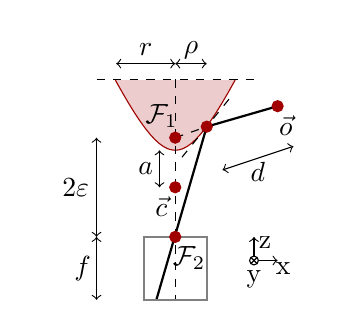
\begin{tikzpicture}[node distance=4em, auto]
    % Background size
    \node[background] at (0,-1.1cm) {};

    % hyperbola
    \pgfmathsetmacro{\e}{1.1};   % eccentricity
    \pgfmathsetmacro{\a}{1.1};
    \pgfmathsetmacro{\b}{(\a*sqrt((\e)^2-1)} 
    \draw[red1, fill=red1!20, yshift=-2.0cm] plot[domain=-1.2:1.2, rotate=90] ({\a*cosh(\x)},{\b*sinh(\x)});

	\coordinate (m) at (0.4,-0.6);
    \coordinate (o) at (1.3,-0.34);
    \coordinate (c) at (0,-1.37);
    \coordinate (v) at (0,-0.74);
    \coordinate (f) at (0,-2.00);
    \coordinate (cam) at (-0.24,-2.8);

    % Draw axis
    \draw [-, dashed] (0,0) |- (0,-2.8);
    \draw [-, dashed] (-1,0) |- (1,0);
	\draw [-, dashed] (v) -- (m);
	\begin{scope}[rotate around={51:(m)}]
			\draw[-, dashed] (0.4-0.5,-0.6) -- (0.4+0.5,-0.6);
	\end{scope}

    % Mini-Coordinate-System
    \draw [->] (1.0,-2.3) |- (1.3,-2.3) node [xshift=0.2em,yshift=-0.3em,anchor=center] {x};
    \draw [->] (1.0,-2.3) -- (1.0,-2.0) node [xshift=0.4em,yshift=-0.2em,anchor=center] {z};
    \draw [color=black, fill=white] (1.0,-2.3) circle(0.056) node [below] {y};
    \draw [-] (0.96,-2.34) -- (1.04,-2.26);
    \draw [-] (0.96,-2.26) -- (1.04,-2.34);

    % Light
    \draw[-, thick] (m) -- (cam);
    \draw[-, thick] (m) -- (o);

    % camera
    %\draw [-, thick, gray] (-0.5,-2.0)
    %    -- (0.5,-2.0)
    %    -- (0.3,-2.3)
    %    -- (-0.3,-2.3)
    %    -- (-0.5,-2.0);
    \draw [-, thick, gray] (0.4,-2.0) 
        -- (0.4,-2.8)
        -- (-0.4,-2.8)
        -- (-0.4,-2.0)
        -- cycle;

    % point
    \draw[fill=red1, color=red1] (m) circle (2pt) node [below, color=black, xshift=0.3em, yshift=0.1] {}; % was: $\hat{\vec o}$
    \draw[fill=red1, color=red1] (o) circle (2pt) node [below, color=black, xshift=0.3em, yshift=0.1] {$\vec{o}$};
    \draw[fill=red1, color=red1] (c) circle (2pt) node [below, color=black, xshift=-0.5em] {$\vec{c}$};
    \draw[fill=red1, color=red1] (v) circle (2pt) node [above, color=black, xshift=-0.5em] {$\mathcal{F}_1$};
    \draw[fill=red1, color=red1] (f) circle (2pt) node [below, color=black, xshift=0.5em] {$\mathcal{F}_2$};

    % sizes
    \path[<->]
        (-1.0,-0.74) edge node [xshift=-0.75em, anchor=center] {$2\varepsilon$} (-1.0,-2.0)
        (-1.0,-2.0) edge node [xshift=-0.5em, anchor=center] {$f$} (-1.0,-2.8)
        (-0.2,-0.9) edge node [xshift=-0.5em, anchor=center] {$a$} (-0.2,-1.37)
        (0.0,0.2) edge node [yshift=0.5em, anchor=center] {$\rho$} (0.4,0.2)
        (0.0,0.2) edge node [yshift=0.5em, anchor=center] {$r$} (-0.75,0.2)
        (0.6,-1.15) edge node [yshift=-0.5em, anchor=center] {$d$} (1.5,-0.85);
\end{tikzpicture}
